\documentclass[uplatex,dvipdfmx,a4paper,11pt]{jsarticle}

\usepackage{url}
\usepackage[dvipdfmx]{hyperref}

\usepackage[top=25mm,bottom=25mm,left=25mm,right=25mm]{geometry}

\usepackage{array}
\usepackage{tabularx}
\usepackage{booktabs}
\usepackage{enumitem}
\usepackage{graphicx}
\usepackage{longtable}
\usepackage{listings}

\lstset{
  basicstyle=\ttfamily\scriptsize,
  breaklines=true,
  frame=single,
  numbers=left,
  numberstyle=\tiny,
  tabsize=2,
  showstringspaces=false
}

\setlength{\parindent}{0pt}
\setlength{\parskip}{0.6em}

\usepackage{titlesec}
\titleformat{\section}
  {\normalfont\Large\bfseries}{\thesection.}{0.6em}{}
\titleformat{\subsection}
  {\normalfont\large\bfseries}{\thesubsection}{0.6em}{}
\titlespacing*{\section}{0pt}{1.2em}{0.6em}
\titlespacing*{\subsection}{0pt}{1.0em}{0.4em}

\newcommand{\sectionrule}{\par\medskip\noindent\rule{\linewidth}{0.6pt}\par\medskip}

\renewcommand{\labelitemi}{\textbullet}
\renewcommand{\labelitemii}{\textopenbullet}
\setlist[itemize]{leftmargin=1.6em,itemsep=0.1em,topsep=0.2em}
\setlist[enumerate]{leftmargin=2.0em,itemsep=0.1em,topsep=0.2em}

\providecommand{\textopenbullet}{\ensuremath{\circ}}


\begin{document}


{\LARGE\bfseries 作業ログ}\par\bigskip

報告者：佐藤涼菜

報告日：7月1日

プロジェクト名：マジカル☆観覧車

\sectionrule


\section{進捗サマリー（要約）}

\begin{itemize}
  \item 全体進捗率：95[％]
  \item マイルストーン達成状況：テストフェーズの結合テストを実施
  \item 主要成果：
    \begin{itemize}
      \item {結合テスト（No.3121, 3141, 3211, 3212）を実施}
      \item {計画書との変更履歴および計画書の訂正を完了}
      \item {LEDマトリクスの反映確認（No.3241）を完了}
    \end{itemize}
  \item 重大課題（影響度：高）：
    \begin{itemize}
      \item {特になし}
    \end{itemize}
\end{itemize}

\sectionrule


\section{作業ログ（詳細トラッキング）}

\subsection{作業ログ}

\renewcommand{\arraystretch}{1.2}

\small

\begin{longtable}{|c|p{2.2cm}|c|c|c|c|p{2.4cm}|p{3.1cm}|}
\caption{作業ログ} \\
\hline
No. & 作業項目 & 開始日 & 予定完了日 & 状態 & 進捗率 & 依存関係・ブロッカー & コメント \\
\hline
\endfirsthead

\hline
No. & 作業項目 & 開始日 & 予定完了日 & 状態 & 進捗率 & 依存関係・ブロッカー & コメント \\
\hline
\endhead

\hline
\multicolumn{8}{r}{次ページへ続く} \\
\hline
\endfoot

\hline
\endlastfoot

3121 &
演奏開始の合図送信確認 &
6/10 &
6/17 &
進行中 &
80\% &
無 &
グループで集まり実施．\\
\hline

3141 &
レーザー受信確認 &
6/17 &
7/1 &
進行中 &
80\% &
無 &
グループで集まり実施．\\
\hline

3211 &
開始信号の受信確認 &
6/10 &
6/17 &
進行中 &
80\% &
無 &
グループで集まり実施．\\
\hline

3212 &
BPM・音量変化の反映確認 &
6/10 &
7/1 &
進行中 &
80\% &
無 &
グループで集まり実施．\\
\hline

3241 &
LEDマトリクスの反映確認 &
6/17 &
7/1 &
完了 &
100\% &
無 &
結合テストにて確認完了．\\
\hline

- &
計画書の変更履歴・訂正 &
6/25 &
6/25 &
完了 &
100\% &
無 &
変更履歴と計画書の訂正を実施．\\
\hline

- &
作業ログの記入 &
6/30 &
6/30 &
完了 &
100\% &
無 &
特になし．\\
\hline



\end{longtable}


\subsection{日ごとの作業ログ}
 今週は6/25,6/30の放課後にてグループで集まり，結合テストを実施したことが主な作業として挙げられる．なお，ガントチャートに結合テストに該当する作業項目が存在しないため，今回は代替としてNo.3121,No3141,No3211,No3212に
 加算している．また，この2日間の作業時間は，各作業項目の時間を明記することが困難であったため，グループで結合テストを実施した合計稼働時間とした．したがって，今週の合計作業時間は16hである．


    \renewcommand{\arraystretch}{1.2}

    \small

    \begin{longtable}{|c|c|p{2.4cm}|c|c|c|c|p{3.8cm}|}
    \caption{日ごとの作業ログ} \\
    \hline
    日付 & No. & 作業項目 & 時間 & 開始時の状態 & 終了時の状態 & 進捗率 & コメント \\
    \hline
    \endfirsthead

    \hline
    日付 & No. & 作業項目 & 時間 & 開始時の状態 & 終了時の状態 & 進捗率 & コメント \\
    \hline
    \endhead

    \hline
    \multicolumn{8}{r}{次ページへ続く} \\
    \hline
    \endfoot

    \hline
    \endlastfoot

    6/24 & 3141 & LEDMatrixの反映確認 & 1.5h &
    未着手 &
    完了 &
    100\% &
    授業内にて確認完了．\\
    \hline

    6/25 & 3121 & 演奏開始の合図送信確認 & 6h &
    進行中 &
    進行中 &
    80\% &
    グループで集まり通信班の手伝いとして実施．\\
    \hline

    6/25 & 3141 & レーザー受信確認 & 6h &
    進行中 &
    進行中 &
    80\% &
    グループで集まり通信班の手伝いとして実施．\\
    \hline

    6/25 & 3211 & 開始信号の受信確認 & 6h &
    進行中 &
    進行中 &
    80\% &
    グループで集まり通信班の手伝いとして実施．\\
    \hline

    6/25 & 3212 & BPM・音量変化の反映確認 & 6h &
    進行中 &
    進行中 &
    80\% &
    グループで集まり通信班の手伝いとして実施．\\
    \hline

    6/25 & - & 計画書の変更履歴・訂正 & 3h &
    未着手 &
    完了 &
    100\% &
    計画書との変更履歴と計画書の訂正を実施．\\
    \hline

    6/30 & 3121 & 演奏開始の合図送信確認 & 3.5h &
    進行中 &
    進行中 &
    80\% &
    グループで集まり通信班の手伝いとして実施．\\
    \hline

    6/30 & 3141 & レーザー受信確認 & 3.5h &
    進行中 &
    進行中 &
    80\% &
    グループで集まり通信班の手伝いとして実施．\\
    \hline

    6/30 & 3211 & 開始信号の受信確認 & 3.5h &
    進行中 &
    進行中 &
    80\% &
    グループで集まり通信班の手伝いとして実施．\\
    \hline

    6/30 & 3212 & BPM・音量変化の反映確認 & 3.5h &
    進行中 &
    進行中 &
    80\% &
    グループで集まり通信班の手伝いとして実施．\\
    \hline


    6/30 & - & 作業ログの記入 & 2h &
    未着手 &
    完了 &
    100\% &
    特になし．\\

    \end{longtable}

\sectionrule

\section{計画時のGCと現在のGC}

計画段階のガントチャート(GC)を図\ref{fig:gant7}（実装フェーズ）および図\ref{fig:gant8}（テストフェーズ）に示す．

\begin{figure}[htbp]
    \centering
    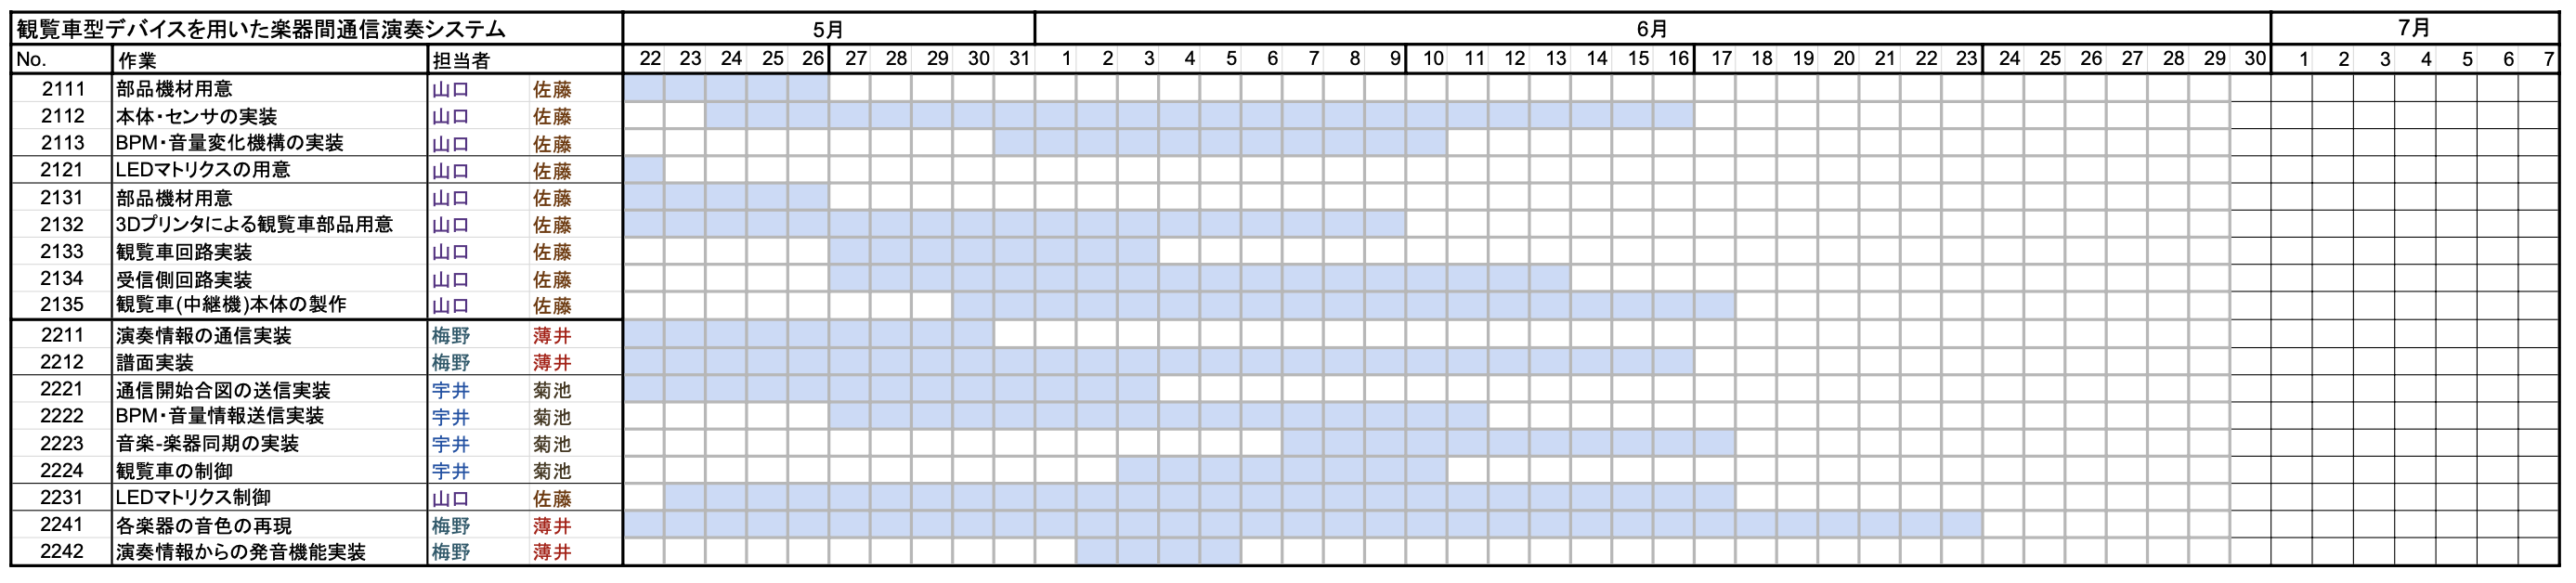
\includegraphics[width=0.9\columnwidth]{gant7.png}
    \caption{計画段階のガントチャート（実装フェーズ）}
    \label{fig:gant7}
\end{figure}

\begin{figure}[htbp]
    \centering
    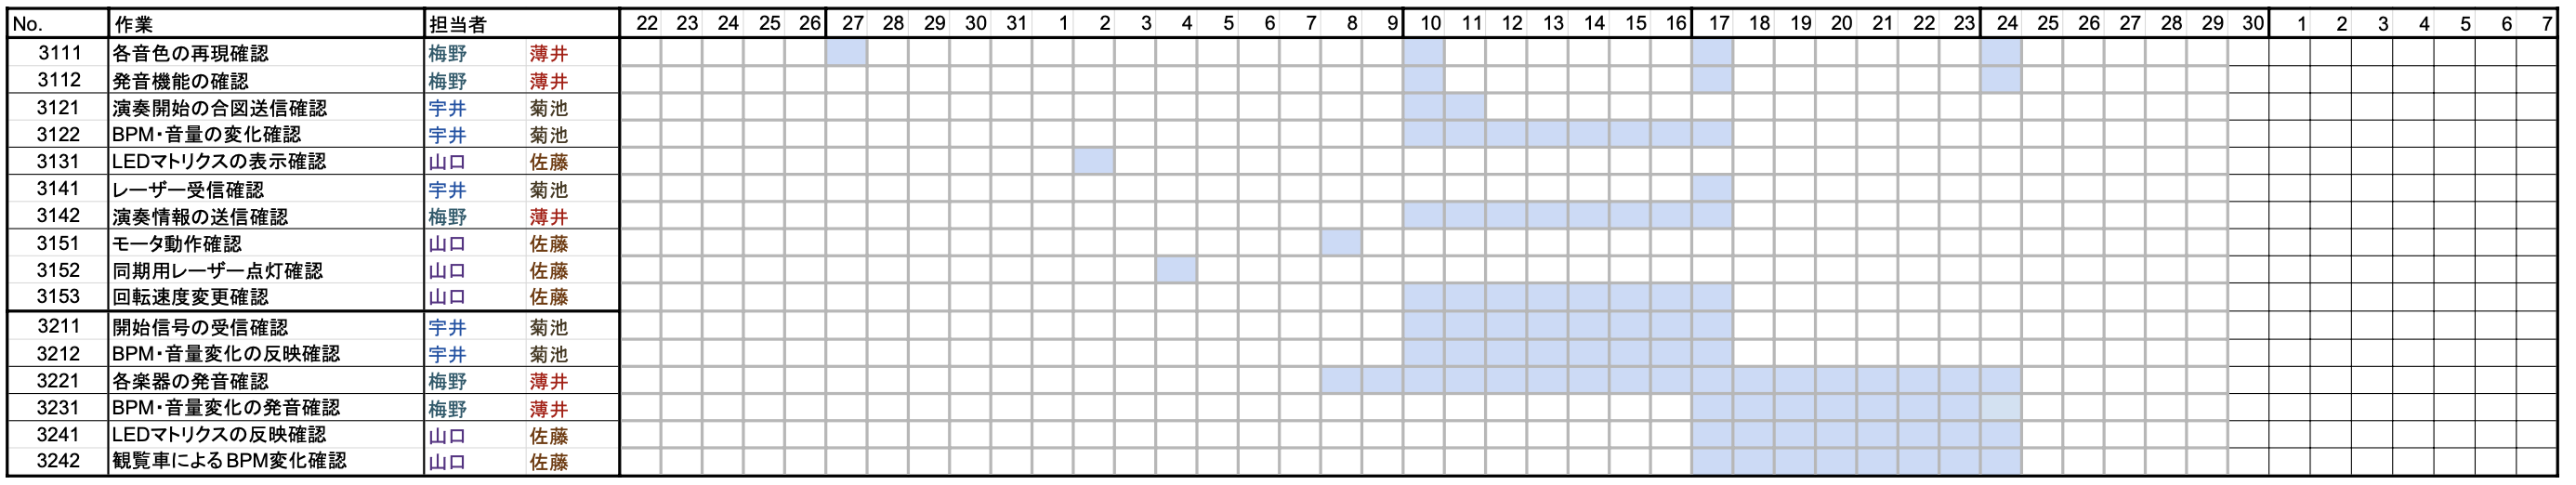
\includegraphics[width=0.9\columnwidth]{gant8.png}
    \caption{計画段階のガントチャート（テストフェーズ）}
    \label{fig:gant8}
\end{figure}

次に，現在のGCを図\ref{fig:gant12}に示す．達成した項目は緑色で塗られている．

\begin{figure}[htbp]
    \centering
    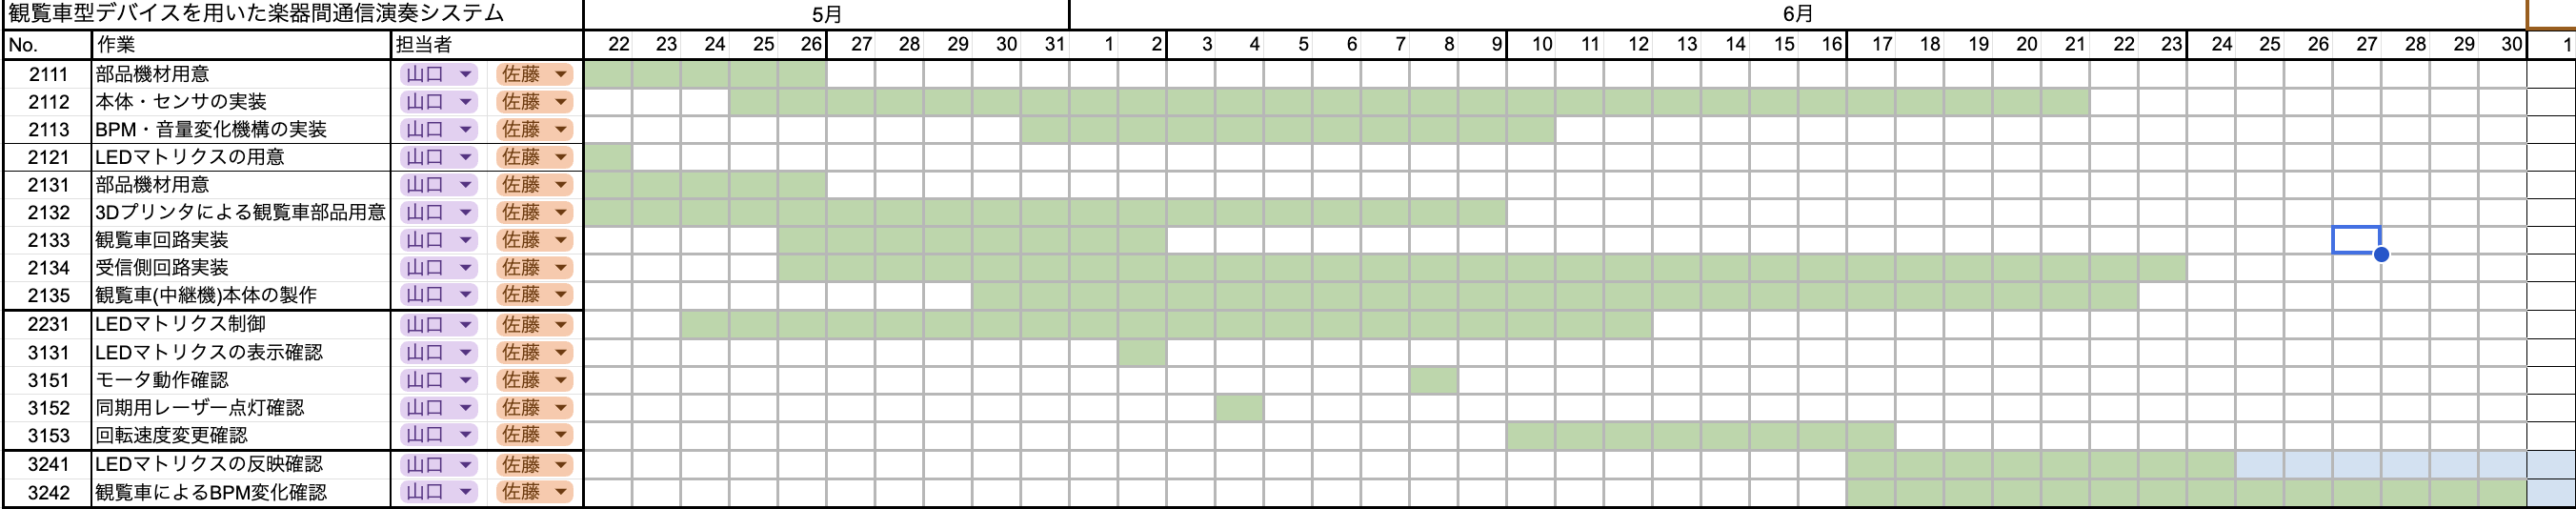
\includegraphics[width=0.9\columnwidth]{gant12.png}
    \caption{現在のガントチャート}
    \label{fig:gant12}
\end{figure}


\sectionrule


\section{課題管理}

\begin{tabularx}{\linewidth}{@{}p{3cm}Xllp{3.2cm}ll@{}}
\toprule
課題 & 発生原因 & 影響度 & 優先度 & 対策 & 期限 & 状態 \\
\midrule
テストフェーズが結合待ち（No.3241に影響） & 通信系との結合が完了していないため，LEDマトリクスの反映確認テストが実施できない． & 高 & 中 & 6/25にグループで集まり結合テストを実施し，確認完了．  & 6/30 & 対応済 \\
\bottomrule
\end{tabularx}

\medskip
※影響度＝プロジェクトへのインパクト

※優先度＝対応の緊急性

\sectionrule


\section{AI利用状況と検証（再現性重視）}

今回はAIを利用していない．

\sectionrule


\section{次回計画}


\begin{itemize}

  \item 目標：最終発表に向けた準備
    \begin{itemize}
      \item 残りのテスト項目の確認と最終調整を行う．
      \item 発表資料の作成に着手する．
    \end{itemize}

  \item 達成基準：
    \begin{itemize}
      \item 全テスト項目が完了し，システム全体が正常に動作すること．
    \end{itemize}

  \item 期限：
    \begin{itemize}
      \item 2026/7/7
    \end{itemize}

\end{itemize}


\sectionrule


\end{document}
